\documentclass{csspaper}
\卒論
%\修論
% \usepackage{epsbox}
\usepackage{makeidx}
\usepackage[dvipdfmx]{graphicx}
\usepackage{listings,jvlisting}
  \title {調査項目の拡張しやすさを考慮した\\ソースコード解析システムの構築}
   \author{小方 亮人}
   \teacher{香川~考司}
   \year{令和4年度~(2022年度)}
\date{令和5年2月9日}
% \date{\today}

\lstset{
    basicstyle={\ttfamily},
    identifierstyle={\small},
    commentstyle={\smallitshape},
    keywordstyle={\small\bfseries},
    ndkeywordstyle={\small},
    stringstyle={\small\ttfamily},
    frame=single,
    breaklines=true,
    columns=[l]{fullflexible},
   %  numbers=left,
    xrightmargin=3zw,
    xleftmargin=3zw,
    numberstyle={\scriptsize},
    stepnumber=1,
    numbersep=1zw,
    lineskip=-0.5ex
}

\makeindex

% \etitle{Implementation of a Source Code Analysis System Considering the Ease of Expansion of Survey Items}
% 2006/2/7改訂
% タイトルを複数行にしたいときは、下のetitleenv環境を使ってください。
\begin{etitleenv}
   Implementation of a Source Code Analysis System Considering the Ease
   of Expansion of Survey Items.
\end{etitleenv}

\begin{eabstract}
A novice programmer who has just started learning programming
often spends a lot of time fixing errors because she cannot understand
the meaning of errors and warnings.
By outputting easy-to-understand error messages for common mistakes
made by novice users, it is possible for them to understand which
line of the source code is wrong and how to correct errors efficiently.
Also, it is required that the system can easily include
new investigated items. Therefore, in this study, we have
constructed a system to point out incorrect locations on source code
input on a web-based system. The language-c-quote library of Haskell is used
for source code analysis and it is expected to that its survey items
can be easily expanded. By clearly displaying the
line number and how to correct errors, it helps novice learner's
programming learning. For the evaluation, we asked members in our laboratory
to use the system and to answer a questionnaire. Based on the results
of the questionnaire, it is considered useful
as a learning support system. On the other hand,
many issues were found, such as the lack of items
that could be investigated for errors and the separation of the
input screen for the source code and the page for outputting the
analysis result.
\end{eabstract}

\begin{jabstract}
プログラミングを学び始めたばかりの初学者は、コンパイル時のエラーや警告が
何を意味しているのかが分からずエラーの修正に時間をかけてしまうことが多々ある。
初学者によくある間違いに対して分かりやすいエラーメッセージを出力することにより
ソースコードの何行目がどう間違っているのかが理解でき、
効率的に修正を行うことができる。また、新しく調査したいエラー項目ができた場合に
システムに組み込みやすいことが求められる。
そこで本研究では、Webベース上で入力されたソースコードに対して
間違っている内容を指摘するシステムを構築した。ソースコードの解析には
Haskellのlanguage-c-quoteを用い、調査項目の拡張性が期待できる。
エラーのある箇所の行番号や修正方針を分かりやすく表示することで
初学者のプログラミング学習を支援する。
研究室の学生に実際に使用して評価をしてもらい、その結果から
エラー箇所や内容の表示は学習支援システムとして有用であると考えられる。
一方で調査できるエラー項目が少ない点、ソースコードの入力画面と
解析結果の出力を行うページが分かれている点といった課題点が
多く残っていることも分かった。
\end{jabstract}


\begin{keyword}
Haskell,構文解析,プログラミング学習支援,ソースコード解析
\end{keyword}

\begin{document}
\maketitle
%  \listoffigures % 図の目次
%  \listoftables  % 表の目次

   \chapter{はじめに}
      \section{研究背景}
      大学で情報系の専攻に進むとプログラミングを学習する機会が訪れるが、
      高校生までにプログラミングを行ったことがある経験者は少なく、
      大学に入ってから初めて学習するといった学生が多い。
      本学部では一年次後期にプログラミングの講義があるが、
      初めからソースコードに間違いもなくすらすらと課題をこなしていく学生は一握りである。
      プログラミングを学び始めたばかりの初学者は、
      幾度となく表示されるコンパイルエラーを見ながら
      自分が記述したコードの間違っている箇所を修正する作業を繰り返すことになる。
      しかし、初学者にはコンパイルエラーや警告が何を意味しているのかが分からず、
      エラーの修正に多くの時間をかけてしまうことが多々ある。
      また、エラーの中にはコンパイル時にエラーとして出力されない
      インデントのミスといったものも含まれる。
      そのような初学者にこそ数多く起こりがちなミスに対して、
      まだプログラミングを始めたばかりの学習者が自力で対応することは困難である。
      学習を続けるにつれて慣れていくものではあるが、初めはエラー表示の示している内容を
      いちいち調べて理解していく必要がある。
      その調子ではプログラミング学習の進む速度は遅く、
      かといって毎回教育者にエラーの内容を聞くことは
      学習者にとっても教育者にとっても負担となる。
      これは学習者に対してプログラミングへの苦手意識を抱かせることに繋がり、
      その苦手意識がその後のプログラミング学習へ悪影響を与えることは容易に想像できる。
      この問題を解決する方法として、初学者によくある間違いに対し
      より分かりやすいフィードバックを即座に出力することにより、
      エラーの修正方針が立てやすくなり、無駄な時間を削ることで、
      学習効率を向上させることができる。

      この方法に取り組んだ研究として、C-Helper \cite{1,2,3}や
      これを用いた島川の研究 \cite{4}が挙げられる。
      しかしこれらは実装にJavaを用いており、構文解析結果である構文木を
      扱う際にvisitorパターンというデザインパターンが用いられているため、
      データ構造に変化が生じる場合は新しいメソッドの追加と
      各クラスにそのメソッドに応じた実装を追加する必要がある。
      そのため調査できる項目の拡張性に優れていない。

      C-Helperと島川の研究の拡張性に優れていないという問題点に対して
      Haskellによる構文解析を用いることで解決を試みた研究が木村の研究 \cite{5}である。
      木村の研究はソースコードのエラー箇所をハイライトすることによって
      教育者の添削を支援するものである。しかし学習者に対して即座にミスの
      フィードバックを示すことはできず、教育者に対しても実際に目視で確認し
      コメントを付け足す必要があるため完全な自動化は図られていない。

      そこで本研究では、Haskellを用いることで調査項目の拡張性を保持しながら、
      学習者に即座にフィードバックを行うことができるシステムの構築を目標とする。
      調査するソースコードに用いられるプログラミング言語は、
      本コースのプログラミングの講義でも初めに学習するC言語を対象とする。
      またシステム導入の負担をできる限り削減し、プログラムの組み込みや修正が
      行いやすいようにWebベースでの実装を目指す。

      \section{関連研究}
         \subsection{C-Helper}
         C-Helperとは、東京工業大学の内田公太が開発したC言語初学者向けの静的解析ツールである。
         ソースコードの問題点を分かりやすいエラーメッセージとして表示し、
         解決策も提示することでプログラミング学習を支援するシステムである。
         C-Helperが調査できるエラー項目は以下のとおりである。
         \begin{itemize}
            \item インデントの乱れ
            \item printfのパラメタ間違い
            \item scanfの値渡しのミス
            \item returnの記述漏れ
            \item char型変数への文字列の代入
            \item 識別子の重複
            \item 定義されていない関数の使用
            \item 構造体のセミコロン忘れ
            \item 関数定義の余分なセミコロン
            \item 警告を抑え込むキャスト
            \item メモリリーク
            \item 動的に確保した配列に対するsizeof
            \item ヘッダファイルでの実態定義
         \end{itemize}
         しかし、C-HelperはC言語の開発環境として広く使われているわけではない
         Eclipseのプラグインであるためシステムの導入に手間がかかることに加え、
         特定のEclipseのバージョンでしか使用することができないという問題点がある。

         \subsection{C-Helperを用いたWebベースのC言語開発環境の構築}
         島川の研究であるこのシステムでは、C-Helperの導入に関する問題点に対して
         C-Helperの機能をWebベースで利用できるようにすることで解決を試みている。
         もともとEclipseのプラグインであるC-Helperの、Eclipseに依存している
         ライブラリやそのライブラリを使用しているメソッドを書き換えることで
         ソースコードの解析や解析結果の出力部分をWeb上で行えるように変更している。
         しかし、C-Helperの機能をWebベースに移植する形で実装しているため、
         C-Helperで調査できない項目に関しては実装することができない。
         調査項目を増やそうとするとC-Helperのシステムに変更を加えた上で
         このシステムにも実装させるという無駄な手間がかかってしまう。

         \subsection{構文解析を用いたC言語指導コメントシステムの構築}
         木村の研究であるこのシステムは、構文解析を用いてC言語指導コメント支援を
         行うことによりプログラミング指導者を支援するシステムである。
         タブレット型端末上での使用を想定しているため、Webベースでの開発を行い、
         構文解析によって特定の構文や条件式を選択することで、指摘したい箇所の特定を
         素早く行うことができる。
         しかし、長いソースコードでは指摘したい箇所への位置まで移るのに手間がかかる点、
         同一構文内に複数の指摘を行った場合指摘コメントが分かりにくい点といった、
         学習者に即座にフィードバックを表示するうえでの課題点が存在する。
      
      \section{Webベースシステムの利点}
      本研究で構築したシステムは、Webページの入力フォームに
      ソースコードを入力することでサーバに送信され、
      同じくWebページに解析した結果を出力する、
      Webベースのシステムである。
      システムをWebベースにすることによって利用者に
      以下のような利点があると考えられる。

      \begin{itemize}
         \item システムのインストールを行う必要がない
         \item Webブラウザがあればシステムを利用することができる
         \item 常に最新のシステムを利用することができる
      \end{itemize}

      また、開発側にも以下のような利点が考えられる。

      \begin{itemize}
         \item システムの導入に関する手順を説明する必要がない
         \item システムの改良や不具合の修正が行いやすい
      \end{itemize}

      特にシステムの導入に関する負担が双方ともに
      軽減されることに繋がり、気軽にシステムを
      利用することができる。

      \section{静的解析の利点}
      本研究のシステムではソースコードの静的解析を行う。
      静的解析とは、コンピュータのソフトウェアの解析手法の一種であり、
      実行ファイルを実行せずに解析を行うものである。
      反対に、ソフトウェアを実行して行う解析を動的解析と呼ぶ。
      静的解析を行うことでソースコードの記述段階で
      エラーを見つけられ、動的解析よりも早い段階での
      改良が行えるようになる。また、ソースコードの静的解析を行うことは
      学習者がインデントのルールに従うといったコードの可読性を
      高める記述ができるようになることに繋がる。
      それによりコードの誤読による内容の誤解を防ぎ、
      予期しないミスやバグの修正が比較的容易になるなどの利点が考えられる。

      \section{本研究に求められること}
      これらの点を踏まえて、本システムに求められる要件は以下のとおりである。
      \begin{itemize}
         \item 初学者向けの静的解析を行うことができる
         \item 学習者に即座にフィードバックを行うことができる
         \item 調査項目の拡張性が期待できる
         \item Webベースのシステムである
      \end{itemize}
      プログラミング初学者が、自分が記述したソースコードのどの箇所が間違っているのか、
      何が間違っているのか、修正するにはどのようにすれば良いのかを
      理解し、判断することができるために、初学者が陥りがちなエラーに対して
      ソースコードの解析を行い即座にフィードバックを与えることで、
      学習効率の向上に寄与することが期待される。
      また、システムを運用していれば新しく調査項目を追加する必要が出てくる場合があるが、
      その項目を簡単に拡張することができれば、システムの対応できる幅が広がる。
      多くの問題に対処することができるようになることで学習者からの
      要望も応えやすくなり、利用者が増えることに繋がる。
      そして学習者が容易にシステムを利用することができるように
      Webベースでシステムを実装することが求められる。

      \section{章構成}
      本論文の構成は以下のようになっている。
      第2章で本システムを実装するにあたって使用した技術について説明する。
      第3章では実装したシステムについて述べる。
      第4章では本システムの試用実験と評価について述べる。
      第5章で本論文のまとめと課題点について述べる。

   \chapter{使用技術}
   ここでは本システムに使用した技術について説明する。

   \section{Haskell}
      \subsection{Haskellとは}
      Haskellは、計算や処理などを関数の定義の組み合わせとして数学的に扱い記述を
      行っていく関数型言語の1つである。言語の名称は記号論理学者の
      Haskell Brooks Curry 氏に由来している。
      現在主流として用いられている処理系はGHC (Glasgow Haskell Compiler) である。

      \subsection{Haskellの特徴}
      Haskellには参照透過性や遅延評価、静的型付けといった関数型言語に多く採用されている
      機能に加え、パターンマッチや型推論、モナドなどの特徴的な機能がある。
      これらの機能を組み合わせることで命令型言語に比べてHaskellはより簡潔かつ容易に
      関数を実装できることが多い。
      以下にHaskellの特徴的な機能の例を示す。
      \begin{itemize}
         \item 参照透過性
      
         C言語やJavaなどの命令型の文法を持っている言語では、
         プログラミングで解決したい課題に対して、
         命令や命令をひとまとまりにした手続きを組み合わせて記述していく。
         命令の組み合わせによってシステムの状態を変更しているため、
         複数の処理で同じ変数を参照している場合予期していない結果が出力されてしまうことがある。
         これはプログラミングの副作用と呼ばれる。
         Haskellを含む関数型言語ではプログラミングの目的に着目し、
         その目的に沿った関数を定義していくことで記述を行う。
         関数型言語にはプログラミングの副作用を基本的に排除する考えがあり、
         同じ引数で呼び出した関数が返却する値は常に同じ値になるという数学的な
         特徴がある。これを参照透過性といい、いつ関数を呼び出しても同じ結果を返すことが
         安全なプログラムの構築に寄与する。

         \item 遅延評価
      
         一般的なプログラミング言語の場合、関数を呼び出す前に引数が評価され
         その結果が関数に渡されるという正格評価が用いられている。
         しかしHaskellでは引数の値が必要になる時まで評価が行われない特徴がある。
         これを遅延評価といい、関数の引数を参照するときだけでなく変数の値を
         参照する際にも行われる。無限リストの扱いに優れているため、
         主に無限リストから値を取り出す際に用いられることが多い。

         \item パターンマッチ
         
         Haskellの関数は実行時の引数の値に応じて
         関数の処理を場合分けして定義することができる。
         関数を呼び出した際は、関数定義の上から順番に
         引数とパターンを照合し、パターンにマッチした定義の
         右辺の処理が実行される。
         引数がどのパターンにもマッチしない場合エラーが表示される。
         以下の引数の階乗を返却する関数の例では、関数factの引数が0の場合
         返却値は1となり、0でない場合はnに引数が束縛される。

         \begin{lstlisting}
         fact 0 = 1
         fact n = n * fact (n - 1)
         \end{lstlisting}

         \item 型推論
      
         コンパイル時にデータ型を判定する機能を型推論と呼ぶ。
         静的型付けはコンパイルの段階で事前にエラーが発見できる代わりに
         あらかじめデータ型を指定する必要があり、プログラムの
         複雑さや冗長さの原因となってしまう。
         動的型付けはデータ型を指定する手間が省ける代わりに
         実行するまでエラーが分からないというデメリットがある。
         Haskellの型推論は、与えられたコードからコンパイラが
         自動的に型を推測して判断することができる。
         型推論の機能を用いることでデータ型を指定しなくても
         コードを書くことができ、コンパイルの段階で間違いを
         発見することが可能なことで、コードの簡潔な記述と
         エラーの発生を抑えることの両方を実現している。

         \item モナド
         
         モナドとは、Haskellで変数などの値といった、状態を変更する
         破壊的代入や入出力といった様々な言語におけるプログラミングの副作用を
         扱うための方法である。そういった副作用という特徴の型は
         共通の構造を持ち、同じ構造の演算子で扱うことができる。
         その共通の構造を持つ型がモナドと呼ばれる。
         中でもよく用いられるのがIOモナドである。主に入出力に関する
         役割を担うIOモナドを用いた例を以下に示す。

         \begin{lstlisting}
         main :: IO ()
         main = do
                    line <- getLine
                    putStrLn line
         \end{lstlisting}

         上記のコード例では、getLineで標準入力から取得した文字列を
         lineに束縛し、putStrLnの引数に入れている。
         putStrLnはStringを引数としてIOアクションを返す関数であり、
         標準出力への表示を行う。

      \end{itemize}   

   \section{Haskell関連技術}
      \subsection{GHCup}
      GHCup \cite{6}はGHCとその周辺ツールのインストールや
      バージョン管理を行うツールである。
      周辺ツールにはCabal、HLSといったものが含まれる。
      GHCupでは複数のバージョンを管理することができるため、
      最新版のGHCを使用したり、最新のGHCに対応していないツールを
      利用するためにあえて古いバージョンのGHCを
      用いたりすることができる。
      コマンドghcup listによって何がインストールされているかを
      確認することができる。

      \subsection{Cabal}
      Cabal \cite{7}はHaskellのライブラリとプログラムを、
      ビルド及びパッケージ化するためのシステムである。
      パッケージの作成者と配布者がアプリケーションを移植可能な方法で
      容易に構築することができるように共通のインタフェースが定義されている。
      本システムではシステムプロジェクトの作成及び
      必要なライブラリやパッケージのインストールにCabalを用いている。

      \subsection{HLS}
      HLS (Haskell Language Server) \cite{8}はHaskellのIDE環境であり、
      Language Server Protocolのためにサーバを実装したものである。
      警告やエラーのハイライト、コードの補完、マウスオーバーによる
      型やドキュメントの表示、定義へのジャンプなどの便利な機能がサポートされている。

      \subsection{language-c-quote}
      language-c-quote \cite{9}はHaskellのライブラリであり、
      一般的なC言語のパーサを提供している。
      language-c-quoteは構文解析\index{こうぶんかいせき@構文解析}の結果が扱いやすいため、
      新しく調査項目を増やす際に容易にプログラムを
      追加することができると考え本システムの構文解析に用いている。
      以下に実際にC言語のソースコードを解析した結果を載せる (図\ref{fig:lcq})。
      その解析結果から調査したい構文等を抜き出し真偽を確かめている。

      \begin{figure}[h]
         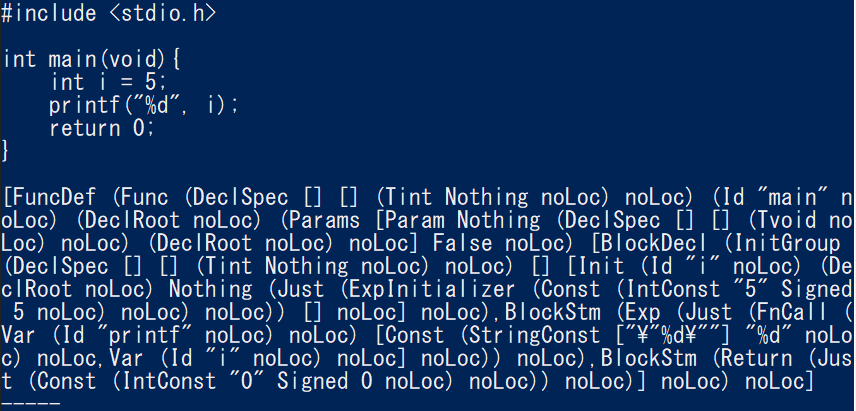
\includegraphics[width=15cm]{lcq.png}
         \caption{language-c-quoteによるソースコードの解析結果}
         \label{fig:lcq}
      \end{figure}

      \subsection{Wai}
      Wai \cite{10}はWebアプリケーションとWebサーバとの間の
      通信プロトコルを提供するHaskellのライブラリである。
      Waiを用いることでWebブラウザ上での入出力と
      サーバ側のHaskellシステムとを繋いでいる。

      \subsection{Warp}
      Warp \cite{11}はWaiをハンドリングするための高速かつ軽量なHTTPサーバである。
      本システムではHaskellプログラム内でのWarpによりローカルサーバを立て、
      ブラウザ上でそこにアクセスすることでシステムの実行を行うことができる。
      以下にWaiとWarpを用いて簡単なWebアプリケーションを作成する方法を載せる (図\ref{fig:warp})。

      \begin{figure}[h]
         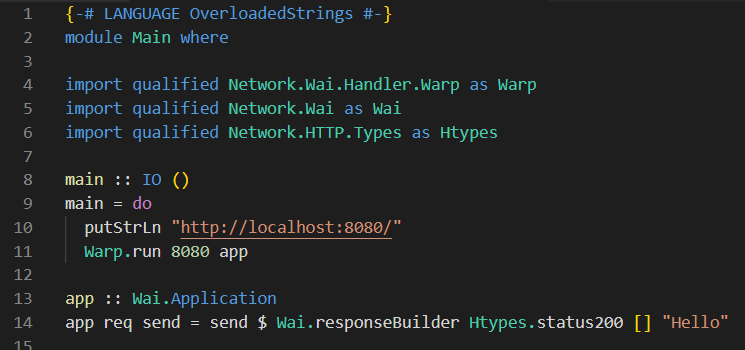
\includegraphics[width=15cm]{wai.png}
         \caption{Wai、Warpによるアプリケーション作成}
         \label{fig:warp}
      \end{figure}

      これをbuildしてrunし、localhost:8080を開くとHelloが表示されている。
   % \section{さぶせくしょん}
   % % 本文開始

   % 卒業論文や修士論文を書くにあたって注意すべき点挙げます.
   % \begin{itemize}
   %  索引\index{さくいん@索引}を必ずつけましょう.
   %  \item 先生方にみていただく前に,推敲しましょう.
   %  \item 参考文献の挙げる順序には,一貫性を持たせましょう.
         %  よくある例としては以下のようなものがあります.
   %   \begin{itemize}
      % \item 論文中での出現順
      % \item 参考文献の筆者の名前順
      % \item 参考文献の出版年月順
   %   \end{itemize}
   %  \item 参考文献の挙げたものは,本文中で言及しなければいけません.
   %  \item 参考文献の例\cite{Thesis2001}
   % \end{itemize}
   \chapter{システムの実装}
   ここでは本システムについて実際の実行画面を踏まえて詳細に述べる。
      \section{システムの概要}
      C言語のソースコードを受け取り、プログラミング初学者が犯しがちな
      間違いを見つけ、ソースコード中の間違っている箇所と
      そのエラーの修正案をそれぞれ提示する。
      プログラミングの学習を支援することで
      初学者がプログラミングに対して苦手意識を持つことを
      防ぎ、効率的に学習を進められるシステムを構築した。
      本研究のシステムはHaskellのプロジェクトであり、
      WaiとWarpを用いることでWebベースでの
      システム構築を行っている。

      本システムの開発環境としては、GHCup 0.1.18.0、
      Cabal 3.6.2.0、HLS 1.8.0.0、GHC 8.10.7を用いている。
      Waiの機能を用い、URLによるルーティング機能が付いた
      サーバを立ち上げる。
      システムを実行するとまず
      ソースコードを入力する画面が表示される。
      ブラウザ上のテキストエリアの
      入力フォームに入力されたソースコードを
      文字列として受け取り、受け取った文字列を
      Haskellのlanguage-c-quoteを用いて
      構文解析を行う。解析した結果から初学者が
      間違いを起こすことの多いif文などの
      情報を抜き出し、間違った記述をしていないか
      調査を行う。そこで間違っている行番号と内容を
      HTMLファイルに出力し、そのファイルを
      ルーティングされた解析結果を表示するページで
      出力する。この出力表示では
      ソースコードの間違っている行番号とその内容が
      一目で分かるように、間違っている行番号の表示を
      他の行と比べて目立つように色を変えている。
      ソースコードの入力画面と出力画面は
      それぞれクリックひとつで即座に
      ページの遷移を行うことができる。
      以下にシステムの概要図を示す。

      \begin{figure}[h]
         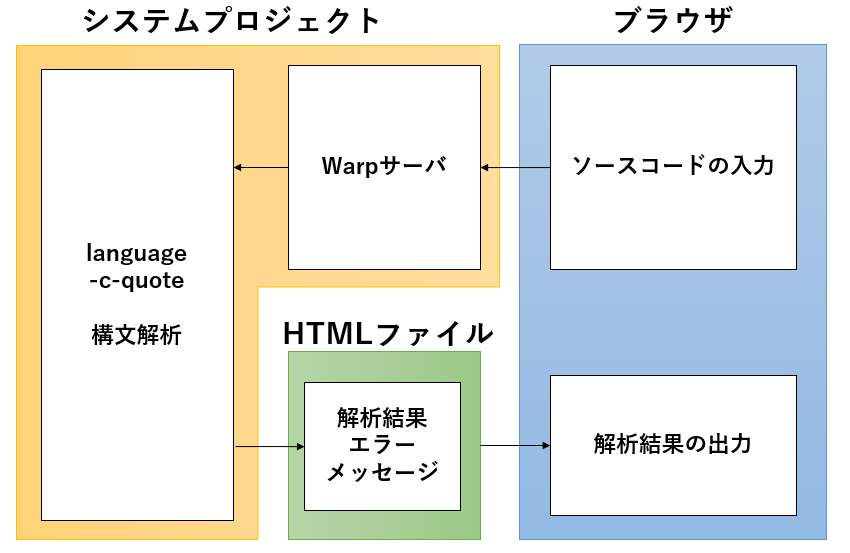
\includegraphics[width=15cm]{system.png}
      \end{figure}

      \section{ソースコードの解析}
      本システムではソースコードの解析にHaskellのライブラリである
      language-c-quoteを用いている。

      \begin{lstlisting}
      import Language.C
      import Data.ByteString.UTF8 as UTF8 (fromString)

      parseProg :: String -> Either SomeException [Definition]
      parseProg str = parse [C11] [] parseUnit (UTF8.fromString str) Nothing
      \end{lstlisting}

      上記のparseProgのような関数を作成し、引数strとしてソースコードの
      文字列を渡すことで構文解析が行われる。
      実際に以下のソースコードを解析した結果を載せる。(図\ref{fig:lcq1})

      \begin{lstlisting}
      #include <stdio.h>
         
      int main(void){
          int i = 5;
          if (i == 5) {
              printf("%d", i);
          }
          return 0;
      }
      \end{lstlisting}

      \begin{figure}[h]
         \centering
         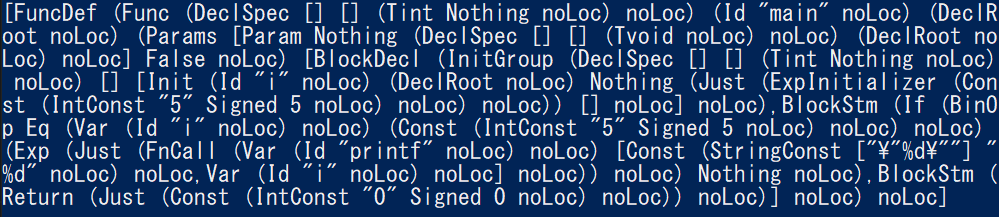
\includegraphics[width=13cm]{lcq1.png}
         \caption{language-c-quoteで解析した結果}
         \label{fig:lcq1}
      \end{figure}

      このような解析結果から調査したい構文や変数等を
      抜き出すことで真偽の判定を行っている。
      図\ref{fig:lcq1}の解析結果から実際に
      if文やprintfの情報を抜き出す方法を以下に述べる。

      language-c-quoteで解析された結果を読み取る際に
      重要なことは、いくつも含まれるデータ型に対してそれぞれの
      コンストラクタを理解することである。
      データ型の種類とコンストラクタは、      
      Language.C.Syntax \cite{12}に詳しく記されている。
      例えば図\ref{fig:lcq1}の初めにあるFuncDefの構成は、
      FuncDef Func !SrcLocとなっている。
      このようにして目的の構文を探す。
      if文が始まっている箇所のデータ型は、
      5行目のBlockStmから始まる部分に当てはまっている。
      Language.C.Syntaxと見比べながら詳しく見ると、
      BlockStmはデータ型Stmから始まり、StmがIfの形を取る場合
      If Exp Stm (Maybe Stm) !SrcLocという構成となっていることが分かる。
      ここではExpには(BinOp Eq (Var (Id ``i" noLoc) noLoc) 
      (Const (IntConst ``5" Signed 5 noLoc) noLoc) noLoc)が含まれている。
      このBinOp EqはVarとConstがイコールであることを示しており、
      元のソースコードのif文の条件式である (i == 5) を解析した部分と対応している。
      if文中のprintfは構成のStmに対応しており、
      解析した結果の (Exp (Just (FnCall (Var (Id ``printf" noLoc) noLoc) 
      [Const (StringConst [``¥``\%d¥""] ``\%d" noLoc) noLoc, Var (Id ``i" noLoc) noLoc] noLoc)) noLoc)
      がprintfの内容を示している部分である。

      本システムではこれらの情報をHaskellのコードによって抜き出している。
      if文の条件式やprintfのパラメタミスといった間違いをこのようにして調査している。
      以下にprintfの情報を抜き出す関数の例を載せる。

      \begin{lstlisting}
      strsearch :: Int -> String -> Int
      strsearch num (x1:x2:xs)
        | (((x1 == `\%') && (x2 == `d')) == True) = strsearch (num+1) xs
        | otherwise = strsearch num (x2:xs)
      strsearch num _ = num
      
      myStm :: Stm -> Maybe Int -> Bool
      myStm (Exp (Just (FnCall (Var (Id "printf" _) _) ((Const (StringConst _ str _) _):args) _)) loc) _
        | (strsearch 0 str) == (length args) = True
        | otherwise = False
      \end{lstlisting}

      関数myStmによって解析結果の中からprintfの部分を抜き出している。
      抜き出す際に設定した値のstrとargsにはそれぞれ、
      ``\%d"とVar (Id ``i" noLoc) noLocが含まれている。
      複数の変数が指定されている場合、
      ``\%d \%d"や (Var (Id ``i" noLoc) noLoc, Var (Id ``i" noLoc) noLoc) が値に入る。
      関数strsearchで文字列中の\%dの数を数えることによって、
      (strsearch 0 str)はprintfの書式文字列内で指定されている数を特定している。
      また、argsにはprintfで指定されている変数が複数の場合も含まれているため、
      lengthを用いて変数の数を求めることで、関数myStmは
      printfで記述されている書式文字列内と変数それぞれの
      数が一致していればTrueを返し、一致していなければFalseを返す。
      このようにコードを記述することでprintfの情報を抜き出し、
      間違っているかどうかの調査を行うことができる。
      他の調査項目に関しても同様に、
      解析結果から調査したい構文の部分を抜き出して調査を行っている。
      そのため本システムの調査項目はLanguage.C.Syntaxを理解することで、
      Haskellの知識さえあれば拡張することが可能である。

      \section{調査可能な項目}
      本システムで調査することができる、初学者が犯しがちな間違いを
      以下に述べる。それぞれミスの例を載せ、エラー表示の文を示している。
      % また、エラーメッセージの出力についての説明を記している。
      \begin{itemize}
         \item インデントのミス
         
         インデントについては別項目で詳しく説明する。

         \item printfの変数の数が間違っているミス
         
         \begin{figure}[h]
            \centering
            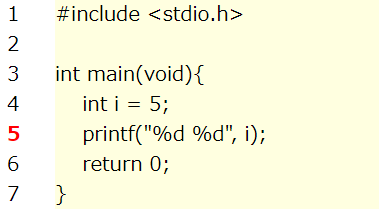
\includegraphics[width=7cm]{sample1.png}
         \end{figure}

         エラー表示:5行目 printfで指定されている変数の数が違います。

         printfで変数を表示する際、第1引数の書式文字列内で
         「\%」記号と変数の型を表す変換指定子を用い、
         第2引数以降に変数を指定することで表示させている。
         書式文字列内と変数それぞれで指定した数が違う場合
         エラーメッセージが表示される。
         現状対応している変換指定子は「d」のみである。

         \item scanfの変数の数が間違っているミス
         
         \begin{figure}[htbp]
            \centering
            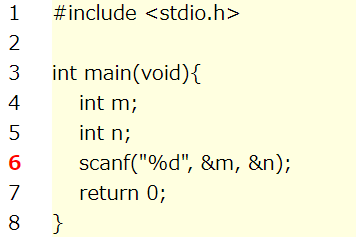
\includegraphics[width=7cm]{sample2.png}
         \end{figure}

         エラー表示:6行目 scanfで指定されている変数の数が違います。

         printfと同様変数を指定する際に、
         第1引数の書式文字列内で「\%」記号と変数の型を表す
         変換指定子を用い、第2引数以降に変数を指定する。
         書式文字列内と変数それぞれで指定した数が違う場合
         エラーメッセージが表示される。
         現状対応している変換指定子は「d」のみである。

         \item if文の条件式が関係演算子ではなく代入式になっているミス
         
         \begin{figure}[h]
            \centering
            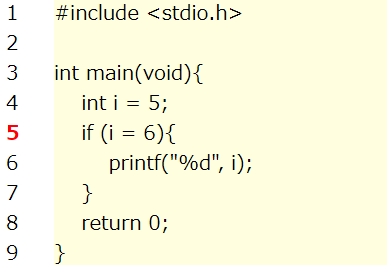
\includegraphics[width=8cm]{sample3.png}
         \end{figure}

         エラー表示:if文の条件式は = ではなく == を使用してください。

         条件分岐を行うif文の条件の部分には関係演算子という
         2つの値の大小関係や等値関係を判定する演算子が用いられる。
         関係演算子には「\textgreater」、「\textless=」などや、
         2つの値が等しいことを示す「==」というものがある。
         これはイコールを2つつなげて等しいことを表しているが、
         間違ってイコールを1つで表そうとしているとエラーメッセージが表示される。
         通常ではif文の条件を記述する部分に代入式を書いても文法的には
         間違っていないためコンパイルが成功してしまうが、
         今回は初学者が間違いに気付けるように
         イコール1つの場合にエラー表示を行うようにした。

         \item 関数名が他の関数と重複しているミス
         
         \begin{figure}[h]
            \centering
            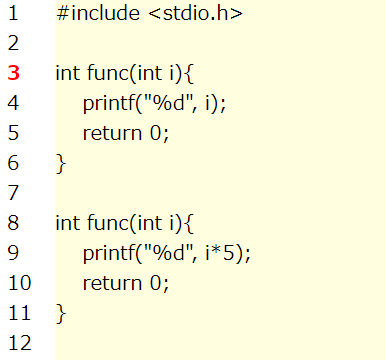
\includegraphics[width=9cm]{sample4.png}
         \end{figure}

         エラー表示:3行目の関数名が他の関数と重複しています。

         定義されている関数の名前が他の関数と
         重複している場合エラーメッセージが表示される。
         関数名の調査はソースコードの上から順番に
         行っているため、重複している二つの関数のうち
         行番号が少ない方の関数のみエラーメッセージの
         表示を行う。また、行番号の強調表示に関しては、
         関数定義の関数名が書かれている箇所に
         強調が行われている。
         
         \item 返却値がint型の関数にreturnが記述されていないミス
         
         \begin{figure}[h]
            \centering
            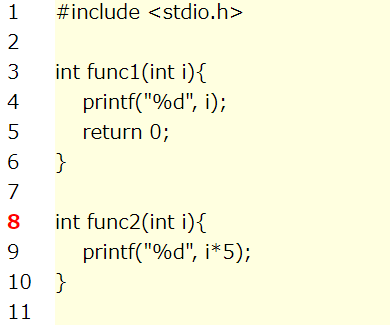
\includegraphics[width=9cm]{sample5.png}
         \end{figure}

         エラー表示:8行目の関数にreturnがありません。

         C言語の関数では戻り値の型を指定して
         関数の定義が行われるが、
         その返却値がint型の場合関数内で
         返却するint型の値をreturnする必要がある。
         そのreturnが行われていない場合、
         エラーメッセージの出力が行われる。
         また、エラー箇所の強調表示は
         その関数の定義が始まっている箇所の
         行番号を強調している。

      \end{itemize}

      \section{インデントのミス}
      ソースコードを記述する際のインデントには様々な方法が存在する。
      本システムで調査するインデントの正しい方法に関しては、
      筆者の指導教員であり、本学で最初にプログラミングを学習する
      講義の担当教員でもある香川が講義で指導している
      インデント方法 \cite{13}を参考として作成している。
      以下に本システムでのインデントルールの特徴的な点について示す。
      \begin{itemize}
         \item 一行に文は一つしか記述しない。
         
         \item 開きブレース「\{」はifやforなどのキーワードと
         同じ行に改行せずに記述する。開きブレースのあとは何も書かずに改行を行う。

         \item 閉じブレース「\}」はifやforなどのキーワードの
         初めの文字と列をそろえて記述する。その行には閉じブレース以外何も書かない。

         \item ブレース「\{ ~ \}」の中は外より空白文字4つ分字下げを行う。
         
         \item 字下げにはタブ文字を使わずに空白文字だけで字下げを行う。
         
         \item if文やfor文などでは、選択されたり繰り返したりされる文が
         一つだけの場合でもブレースで囲んで記述を行う。

         \item 関数の定義は行頭から記述を行う。
         
         \item 余分なブレースは記述しない。
      \end{itemize}

      \begin{figure}[h]
         \centering
         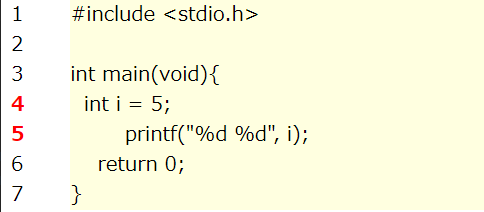
\includegraphics[width=10cm]{sample6.png}
      \end{figure}

      エラー表示:4行目 インデントをスペース2つ分追加してください。

      5行目 インデントをスペース4つ分減らしてください。

      インデントの基準は空白文字4つ分であり、
      それより少ないか多い場合は正しいインデントになるまで変更するべき
      空白文字の数をエラーメッセージとして表示を行う。

      \section{追加できなかった調査項目}
      実装を目指したが実装できなかった調査項目について
      以下に示す。
      \begin{itemize}
         \item for文の書式の間違い
         
         \begin{lstlisting}
         for ( 変数の初期化; 繰り返しの条件式; 変数の変化式 )
         \end{lstlisting}
         
         上記のように、C言語のfor文ではいくつかの式と1つの変数を
         用いて記述を行う。
         まず代入式等を用いて変数に初期値を設定する。
         次に、条件式で繰り返しを続けるための条件を記述する。
         条件式が真の値をとり続けている間はfor文の繰り返しが行われる。
         そのためここでは、「変数の値が0より大きいか」のような
         変数を含む2つの値の大小関係といった式が記述される。
         変化式では繰り返しが行われるたびに、変数に1を足したりといった
         変数の値をどう変化させるかを記述する。
         このように、for文を記述するためには三種類の
         異なる様式の式を用いる必要がある。
         そのため初学者が記述する際に間違いを起こしやすいため
         調査の実装を行いたかったが、
         同じく解析する際も解析結果が複雑になってしまい、
         時間の都合で実装できなかった。
         
         \item if文の中にあるミスの特定
         
         \begin{figure}[h]
            \centering
            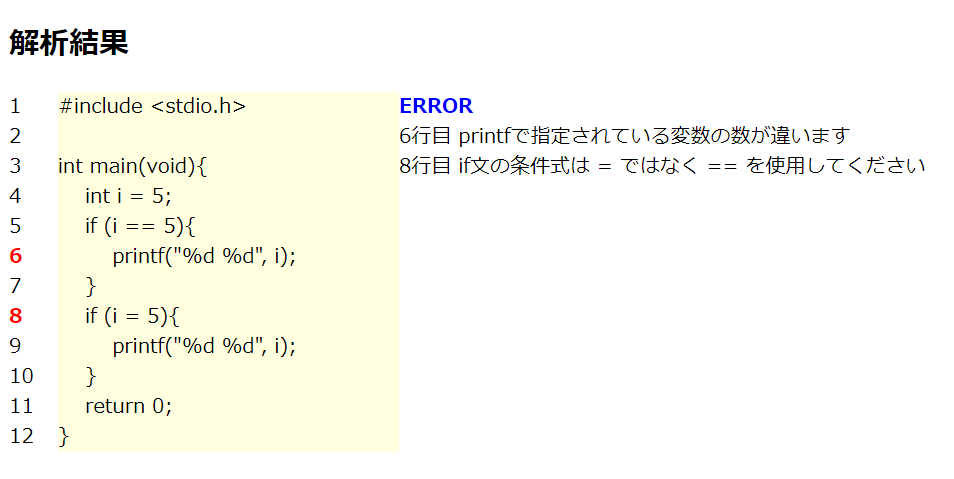
\includegraphics[width=13cm]{sample7.png}
         \end{figure}
         
         上図のように、if文の条件式が成立する場合の処理の中に
         調査可能なミスがあった場合、そのif文の条件式が間違っていなければ
         正確に判定されるが、if文の条件式が間違っていると
         そのミスのエラー判定をしたところでその構文の解析が終了してしまい、
         中の処理部分のエラー判定が行われない。
         そのため修正を挟んで二度システムを実行すればエラーの特定は
         正常に行えるが、最初の実行でif文の条件式と処理との
         両方のエラーを特定できれば修正の手間も一度で済む。
         HaskellのGeneric Programmingに関するライブラリ \cite{14}を用いて、
         間違っている項目が見つかった場合も
         そこで調査を止めることなく、ソースコードの隅々まで
         調査が行えるようにする必要がある。

         \item else文への対応
         
         \begin{figure}[h]
            \centering
            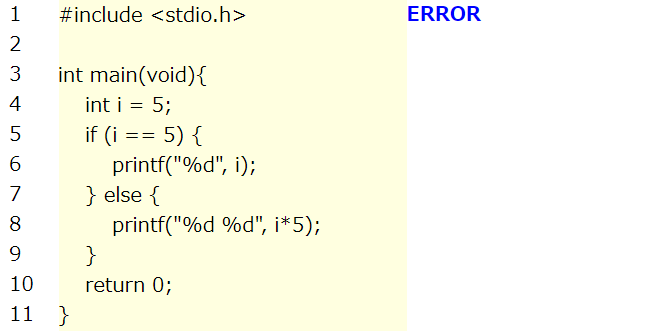
\includegraphics[width=10cm]{sample8.png}
         \end{figure}

         上図の8行目のようにif文の条件式が偽となった場合の処理に用いられるelse文で
         実行される調査可能なはずのエラーの判定が行われない。
         else文にも対応させようとする場合、language-c-quoteで解析された結果を
         Haskellで抜き取る際にif文の情報だけでなく、そこに付随するelse文に関する
         情報も値を設定して格納することで参照することができるようになると考えている。

         \item ソースコード中に日本語がある場合
         
         ソースコード内に日本語がある場合、解析が上手く行われず、
         解析結果の表示がされなくなってしまっている。
         そのためprintfでの日本語表示や
         コメントが含まれるソースコードに対応ができない。
         これはlanguage-c-quoteで解析が行われる際に、
         字句解析によってコードが構文上意味のある最小単位のトークンに
         区切られることが原因と考えられる。
         これを解消するためには、文字列リテラルやコメントに対して
         packを用いてbytestringに変換し、
         エンコードによってUTF-8が含まれているテキストを
         デコードする必要があると考えられる。

         \item 宣言した変数の型と違う型の値を代入しているミス
         
         初学者が起こしがちなミスの一つてして、宣言している変数の型と
         違う型の値を代入してしまうミスが挙げられる。
         例として、以下のソースコードを挙げる。

         \begin{lstlisting}
         int a = 5;
         double b = 3.6;
         int c;
         char d;
         c = a + b;
         d = "string"
         \end{lstlisting}

         この例では、int型の変数cに代入される (a + b) の値はdoubleで行われる。
         そのためint型の変数に代入しようとするとエラーとなる。
         またchar型の変数dには文字列を格納できないためこちらもエラーとなる。
         このように変数宣言時の型によって起こる間違いを特定したいと考えていた。
         そのためには宣言される変数とその型、またそれに代入される
         値の型を全て把握し、照らしあわせる必要がある。

         \item scanfの値渡しのミス
         
         C言語におけるscanfでは第2引数以降に値を格納する変数の記述を行うが、
         C言語では変数に格納された値のコピーのようなものを渡すことしかできないため、
         int型の変数等に入れ込む場合変数のアドレスを渡すことによってscanf関数で
         値の格納を行うことができる。これは変数に「\&」をつける形で記述される。
         しかし文字列を渡す際は配列名に「\&」をつける必要がない。
         これは配列名が配列の最初の要素のアドレスを表していることによるものである。
         この違いは初学者が困惑する項目の一つであり、優先的に実装を行う
         必要がある。

      \end{itemize}

      \section{システムの実行}
      本システムはHaskellプログラム内でのWarpによりローカルサーバを立て、
      そのWebページにアクセスすることでシステムを実行する。
      システムページにアクセスすると、以下の画面が表示される(図\ref{fig:sys1})。

      \begin{figure}[p]
         \centering
         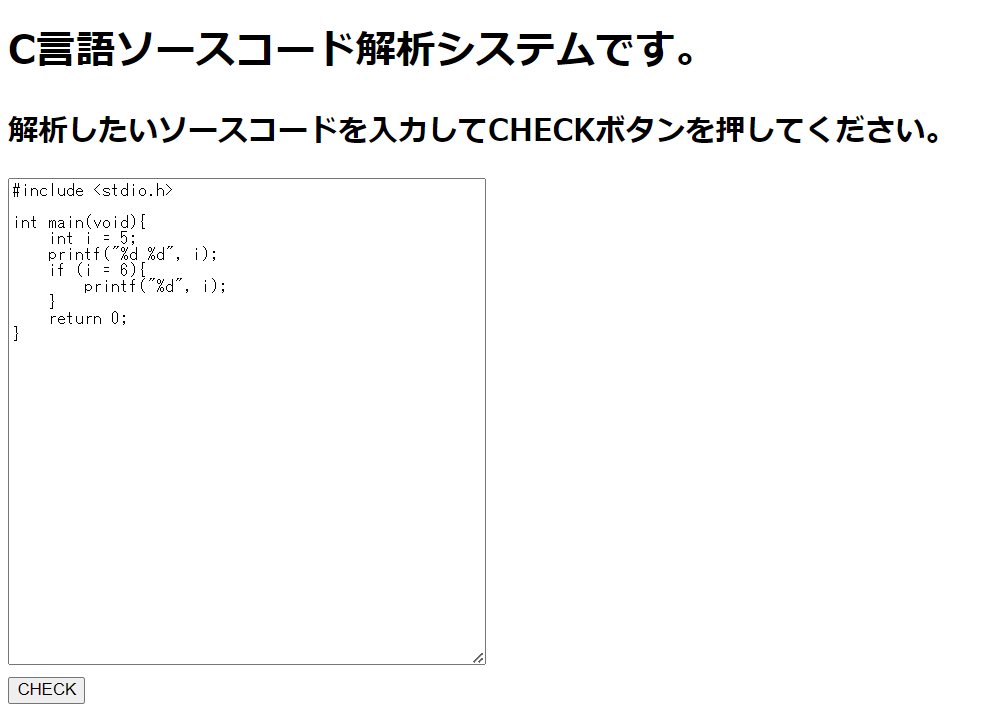
\includegraphics[width=13cm]{systempage1.png}
         \caption{ソースコード入力画面}
         \label{fig:sys1}
      \end{figure}

      表示されているテキストエリアに解析したい
      ソースコードを入力し、CHECKボタンを押すことで
      Haskellプログラムに文字列として
      ソースコードが送信され、構文解析が行われる。
      そして解析した結果とエラーの箇所や内容をHTMLファイルに
      書き込むことで記録する。
      CHECKボタンを押した際にページが結果表示画面に遷移し、
      その書き込まれたHTMLファイルが表示される。
      結果表示の際にはエラーがある行番号の色を変更することで強調している。
      また、左右に分割してコードとエラー内容を表示している。
      実際にソースコードを入力した際の結果表示画面を以下に示す(図\ref{fig:sys2})。

      \begin{figure}[h]
         \centering
         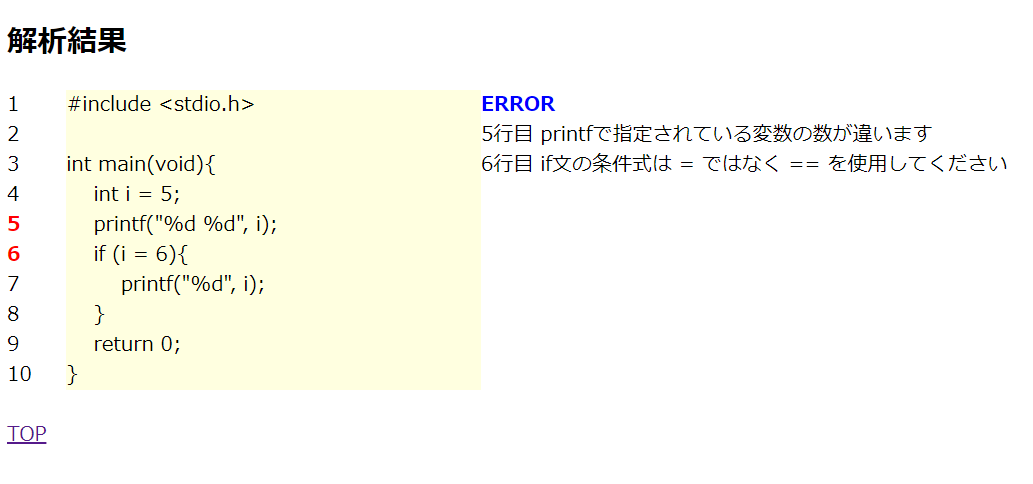
\includegraphics[width=14cm]{systempage2.png}
         \caption{解析結果表示画面}
         \label{fig:sys2}
      \end{figure}

      本システムで調査できる項目の中には、通常のコンパイルでは
      エラーとして認識されないミスもある。
      インデントのミスとif文の条件式のミスがそれにあたる。
      そのため本システムを用いることで通常のコンパイルでは気づけない
      ミスに対してもエラー表示がされ、エラー内容の出力も
      日本語で行われるためそのミスの修正も容易に行うことができる。
      実際に下記のソースコードをコマンドプロンプトでコンパイルした場合(図\ref{fig:sys3})と
      本システムで調査した場合(図\ref{fig:sys4})の結果を示す。

      \begin{lstlisting}[language=c]
      #include <stdio.h>
      
      int main(void){
        int i = 5;
          printf("%d %d", i);
      
          if (i = 5) {
              printf("%d", i);
          }
      
      return 0;
      }

      \end{lstlisting}

      \begin{figure}[p]
         \centering
         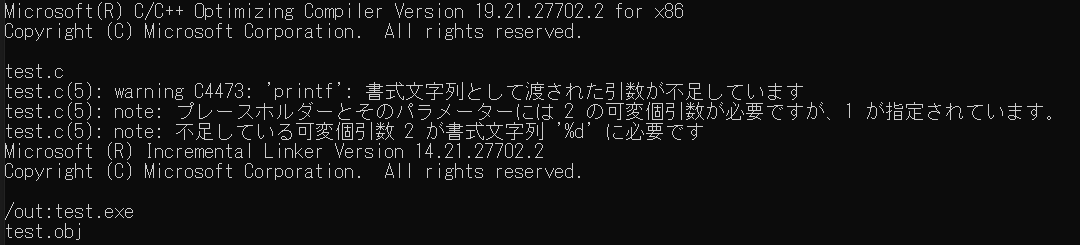
\includegraphics[width=14cm]{compile1.png}
         \caption{コマンドプロンプトでのコンパイル結果}
         \label{fig:sys3}
      \end{figure}

      \begin{figure}[p]
         \centering
         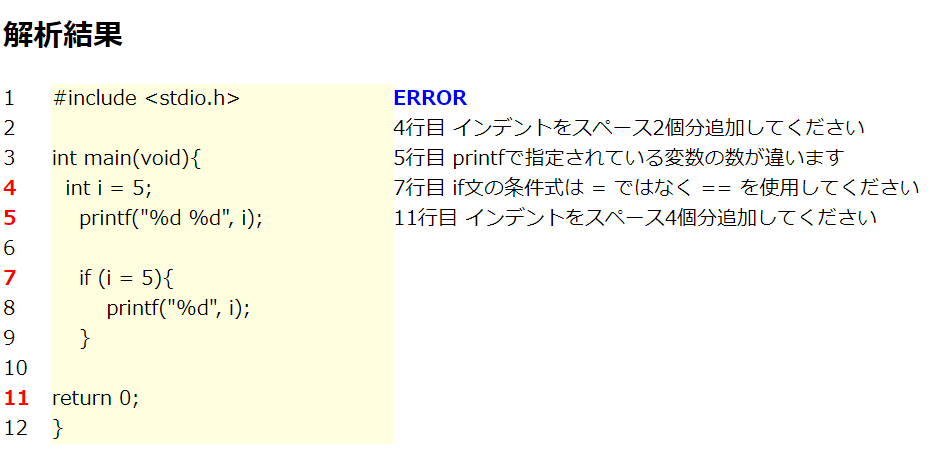
\includegraphics[width=14cm]{compile2.png}
         \caption{本システムでの解析結果}
         \label{fig:sys4}
      \end{figure}

      このように、コマンドプロンプトではインデントのミスやif文の
      条件式に対する警告が表示されていない。
      本システムではそれぞれのミスの箇所と内容を表示させており、
      特にインデントのミスは正しい状態にするためにスペースを
      いくつ追加したり減らしたりすればいいかが表示されているため、
      利用者が自身のソースコードのインデントを容易に整えることができる。

      解析結果の表示画面では特に初学者がソースコードのエラーを
      修正できるように分かりやすくエラー内容を表示することを意識している。
      表示画面の左側では入力されたソースコードを表示させ、
      エラーがある行の行番号は赤色に変更することで一目で間違っている
      行を理解することができる。図\ref{fig:sys3}のコマンドプロンプトの表示では
      エラー内容の表示しか行われていないため、
      視覚的にエラー箇所を理解することができない。
      画面の右側には生じているエラーの内容について行番号と共に記している。
      エラーによっては修正するために何を行えば良いかの表示もしており、
      表示を見てすぐにエラーの修正を行うことができる。

   \chapter{システムの試用実験と評価}
   ここでは、システムの試用実験と評価について述べる。

      \section{システムの試用実験}
      本研究室の学生を対象に、本システムの試用実験を行った。
      実験方法としては、実際に本システムのソースコード解析機能を
      使用してもらい、その後アンケートに回答してもらう形式で行った。
      この試用実験では調査項目の拡張しやすさに関する実験を行うことは
      困難であったため、もう一つのシステムの目的である間違っている箇所の指摘に関連した、
      エラーが起きている箇所が分かりやすいか、
      エラーメッセージによってしっかりと修正を行えそうかという点に
      特に注目して行ってもらった。

      \section{評価項目}
      評価項目に関して、全部で6つの項目を設けた。
      1つ目の項目は、「表示画面は分かりやすいか」という質問である。
      2つ目の項目は、「エラー箇所は分かりやすいか」という質問である。
      3つ目の項目は、「エラー内容は分かりやすいか」という質問である。
      これら3つの質問に対する回答は、1の「わかりやすい」から、4の
      「わかりにくい」までの目盛りを選択するようにした。
      4つ目の項目は、「良いと思う点はどこか」という質問である。
      5つ目の項目は、「悪いと思う点はどこか」という質問である。
      6つ目の項目は、「気になった点、欲しい機能はあるか」という質問である。
      これら3つの質問に対する回答は、自由記述とした。

      \section{結果}

      アンケートの結果を以下に述べる。
      まずは選択式の評価項目について述べる。
      1つ目の項目に対する回答は図\ref{fig:que1}に示すとおりである。
      1番の「分かりやすい」を選んだ回答者と3番を選んだ回答者で大きく2つに分かれている。
      他の2番と4番にはそれぞれ1名ずつが回答している。

      \begin{figure}[htbp]
         \centering
         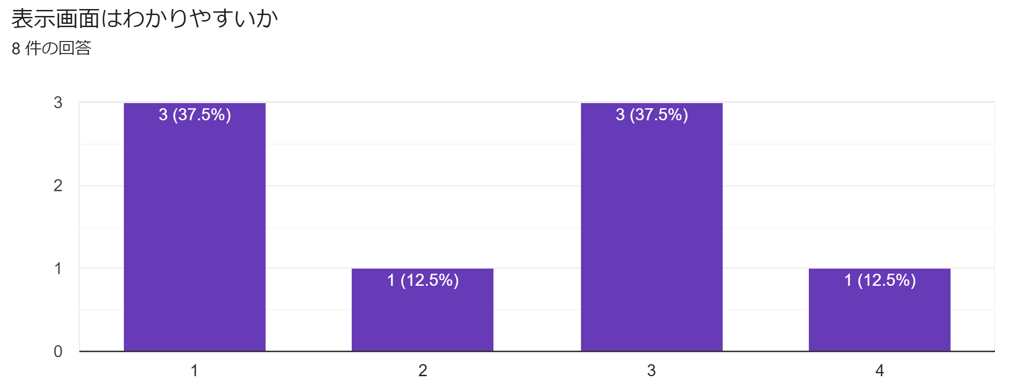
\includegraphics[width=12cm]{question1.png}
         \caption{1つ目の項目に対するアンケート結果}
         \label{fig:que1}
      \end{figure}

      2つ目の項目に対する回答は図\ref{fig:que2}に示す。
      1番の「分かりやすい」を選んだ回答者が過半数を占めている。
      他の2番、3番、4番にはそれぞれ1名ずつ回答している。

      \begin{figure}[htbp]
         \centering
         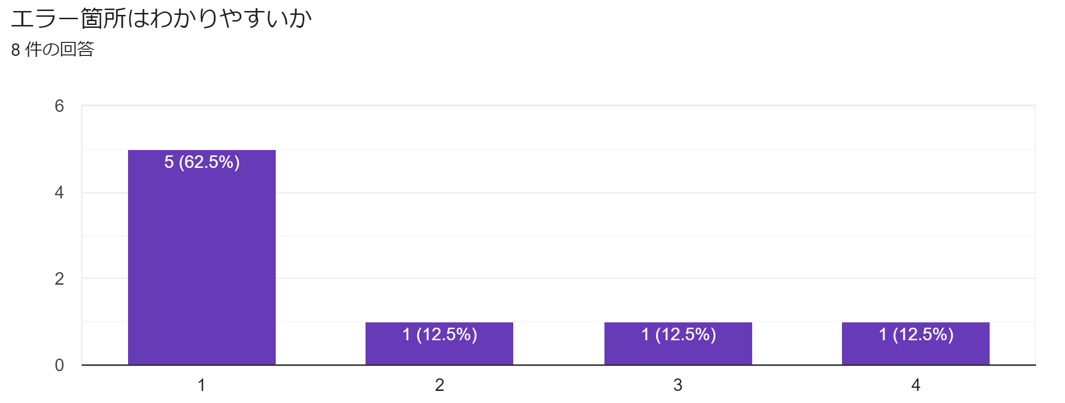
\includegraphics[width=12cm]{question2.png}
         \caption{2つ目の項目に対するアンケート結果}
         \label{fig:que2}
      \end{figure}

      3つ目の項目に対する回答は図\ref{fig:que3}に示すとおりである。
      1番の「分かりやすい」と2番を選んだ回答者が多いことが見て取れる。
      他の3番、4番にそれぞれ1名ずつ回答している。

      \begin{figure}[htbp]
         \centering
         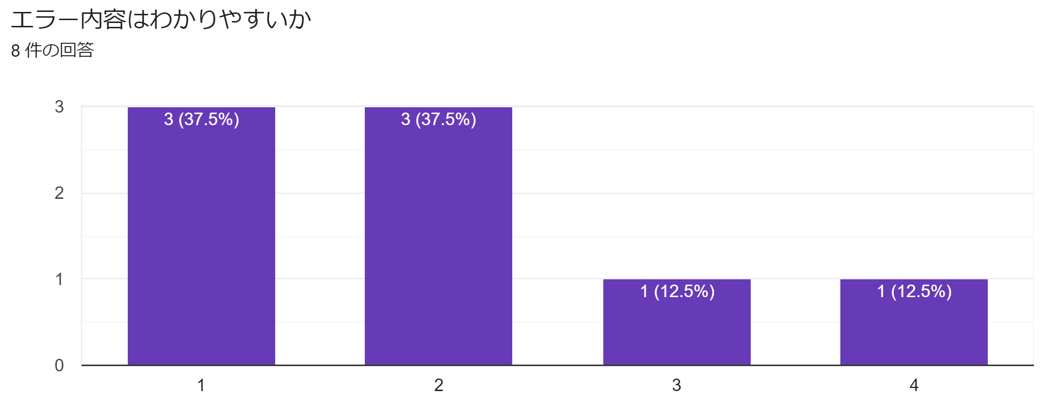
\includegraphics[width=12cm]{question3.png}
         \caption{3つ目の項目に対するアンケート結果}
         \label{fig:que3}
      \end{figure}

      次に、自由記述での評価項目について記す。
      「良いと思う点はどこか」についての回答には以下のような回答があった。

      \begin{itemize}
         \item 修正内容を日本語で出力しているため、分かりやすい
         \item エラーのある行番号の色が変わっているため、修正を行うべき箇所が分かりやすい
         \item システムがシンプルで、操作に迷うことがなかった
         \item 長いコードでも実行速度が速かった
         \item エラーがある箇所の表現が分かりやすかった
         \item 何がどう間違っているのかが具体的だった
      \end{itemize}

      「悪いと思う点はどこか」についてには以下のような回答があった。

      \begin{itemize}
         \item 対応していない要素が多い点
         \item インデントの数は固定せず、変えることができるようにして欲しい
         \item スペルミスがあった場合エラーの検知ができない
         \item 解析結果が別ページで表示される点
      \end{itemize}

      「気になった点、欲しい機能はあるか」という質問には以下のような回答があった。

      \begin{itemize}
         \item エラー箇所の行番号だけではなく、行全体を強調して欲しい
         \item 対応している、していない要素についてシステム内で説明が欲しい
         \item テキストエリアへの入力だけでなく、ファイルで送信したい
         \item インデントのミスをエラーととらえるべきかどうか
         \item 解析結果を見てその場でコードを修正したい
         \item 自動でインデントのミスを修正して欲しい
      \end{itemize}

      \section{考察}
      アンケートの結果から、エラーの箇所や内容に対する評価は「分かりやすい」と
      答えた回答者が多く、本システムがエラーの起きている箇所や
      修正方針を示すことで、初学者がエラーを修正する作業を効率的に
      行うことに寄与できると考えられる。
      しかし、まだ対応していないエラーも多く、
      調査できるエラーとできないエラーについて
      システム内で説明を付け足す必要がある。
      また、結果を表示する画面に関しても課題点が多く、
      特にページが遷移してしまうことで元のコードへの
      修正が行いにくいという意見があった。本システムの開発段階では
      既にエディタ上で記述を済ませているソースコードを
      ペーストすることでの利用を想定していたため、
      そのような点への配慮が欠けてしまっていた。
      そのためソースコードの入力と解析結果の表示は
      同じページ上で行えるようにし、スムーズにコードの修正と解析を
      交互に行えるようにできればより良いシステムになると考えられる。
      また、インデントに関しての意見として、インデントのミスを
      他のエラーと同様の扱いをすることは学生にとって
      印象が良くないのではないかといった意見があった。
      確かにインデントのミスは他のエラーと比べて、
      大きくプログラムの動作に変化が起こるわけではない。
      しかしインデントを整えることでどの行が同じブロックに含まれるのかが
      明示的になり、コードの可読性が上がる。
      自分にとっても他者にとってもコードが読みやすく、
      ミスをしている箇所の探しやすさやプログラムの処理や流れの
      理解しやすさに繋がるため、コーディングにおける重要な項目の
      一つであると考えている。
      そのコーディング時に重視するべきであるインデントは、
      一度自分が行っている記述の仕方に慣れてしまうと
      後から修正を行うことが困難になってしまう。
      そのためプログラミングを始めたばかりの時から
      インデントを意識的に行うようにすることが重要であると考え、
      本システムでも特に重要視している。
      そのインデントのルールには様々な考えがあるが、
      本システムでは既に示したインデントルールにのみ対応しているため、
      字下げの際のスペースの数や改行を行う位置など
      違う方法でのインデントにも対応させることができればと考えている。

   \chapter{結論}
      \section{まとめ}
      本研究では、Haskelによる構文解析を用いてプログラミングを始めたばかりの
      初学者が犯しがちな間違いを特定し、その間違っている箇所と間違いの内容を
      分かりやすく表示させることで、初学者のプログラミング学習を支援する
      システムの開発を行った。Webブラウザ上の入力フォームに解析したい
      ソースコードを入力することで即座にフィードバックが行われる。
      調査可能な項目はHaskellの知識があれば今後も
      あまり手間をかけることなく実装できることが想定される。
      システムをWebベース上で実装しているため、利用者は
      システムの導入作業を行う必要がなく、気軽に利用することができる。
      しかし、構文解析によって調査が行われる項目がまだ少なく、
      解析結果を表示する際にも多くの課題が見つかった。

      \section{今後の課題}
      以下に、本システムの課題点及び解決策を述べる。

      \begin{itemize}
         \item 調査が可能な項目が少ないこと
         
         現状調査可能な項目として、インデントのミス、printfやscanfの
         受け取る変数の数が間違っているミス、if文の条件式が
         関係演算子ではなく代入式になっているミス、
         関数名が他の関数と重複しているミス、
         返却値がint型の関数にreturnが記述されていないミスがあるが、
         これだけでは到底プログラミング学習を完全に
         支援できるとはいいがたい。
         そのため特に初学者が犯しがちなミスについて
         優先的に実装をしていく必要がある。
         実際にプログラミングの講義中に提出された課題を分析し、
         実装するべき項目を精査することも重要である。

         \item ソースコードの入力画面と解析結果の表示画面が別ページであること
         
         本システムでは解析したいソースコードを入力して
         解析を始めると、自動的に別のページに遷移して
         解析結果の表示が行われている。それは学習者にとって
         エラーの修正と解析を繰り返すことのスムーズさに
         繋がるものではない。初学者にとってこのエラーの
         修正作業は何度も行うことになるものであり、
         その点が煩わしいとシステムを利用する機会が
         減ってしまう恐れがある。
         そのため入力画面と解析結果の表示は
         同じページ内で行えるようにすることで、
         容易に自分のソースコードを改善することができ、
         システムの積極的な利用に繋がると考えられる。

         \item 実際に大人数が同時にシステムを利用する実験ができていないこと
         
         本システムが想定しているシステムの利用として、
         学習者がプログラミングの講義を受け、講義中や講義後の課題に
         取り組む際に自身の記述したソースコードが間違っていないか
         確認を行う際に利用されることを想定している。
         特に講義中に出された課題に対して取り組む場合、
         一度に多くの学習者が利用することが考えられる。
         本研究の試用実験は10人程度での実験となっているため、
         実際に何十人もが同時にシステムを利用することになった場合に
         どのようなアクシデントが起こるかが想定できない。
         現状長いソースコードに対しても解析結果の表示が
         素早く行われ、ページの遷移等の動作が重いといった挙動は
         確認されていないが、実際に想定している環境で
         試用実験が行えていないことは課題点である。

         \item Webベースのシステムである利点を最大限に活かせていないこと
         
         本システムは利用者がシステムの導入にかかる負担をできる限り削減する
         ということを目的としてWebベースでシステムの実装を行った。
         利用者はWebページにアクセスするだけでシステムを利用することができるため、
         その目的は達成できているといえる。
         しかし、Webベースシステムの利点を最大限に活かすには他のWebベースのシステムとの
         連携や掲示板のような学習者間でのコミュニケーションが行える機能といった、
         Webベースならではの機能を実装することが必要である。
         例えば他のシステムから本システムのページに対して、
         そのシステムで利用しているソースコードを送信するといった
         システム間のテキスト送受信の仕組みが考えられる。

         \item インデントのエラーを自動で調整する機能を実装すること
         
         初学者にとってインデントのミスは誰しも犯しがちなミスである。
         インデントには様々なルールがあり、正解が一意に定まっているわけではないため、
         初めから正しいインデントを行うことやインデントの修正を行うことは
         プログラミングに慣れるまで難しい。
         そこでインデントのミスを自動的に修正してくれる機能が欲しいという意見があった。
         正しいインデントにするために追加したり減らしたりするスペースの
         数を特定することはできているため、実際にそのスペースの増減を
         反映したソースコードを出力することは可能であると考えられる。
         これは本システムにおける構文解析によってエラーを出力する機能とは
         別の機能として実装することになり、システム自体に
         複数の機能を持たせることができるようになる。

         \item 調査項目の拡張性に関する評価が主観的であること
         
         本システムの目的として、新しく調査したいエラー項目ができた際の
         調査項目の拡張しやすさというものがあった。
         しかしソースコードの解析結果から情報を抜き出すにはHaskellや
         language-c-quoteの知識が必要であり、
         調査項目の拡張性に関しての試用実験を行うことが困難であった。
         そのため拡張性に関しての評価は筆者の主観的なものでしかない。
         そこで、本学にはHaskellを学ぶ講義があるためその講義内で調査を行う
         コードを記述する課題を出したり、知識がなくても調査の
         イメージがつかめるように分かりやすさを重視した
         ビジュアルプログラミングを利用したりといった方法が考えられる。

      \end{itemize}

\acknowledgment  % 謝辞
本研究においてご指導を承りました香川考司先生に心から感謝の意を表します。
そして、本研究のシステム開発や試用評価にご協力いただいた本研究室の藤井陸さん、平西宏彰さん、
大山哲平さん、濱井柚任さん、鎗分汰地さん、MUHAMMAD SULAIMI BIN SABUDINさん、
木野誠真さん、田中舜さん、軒原峻維さん、SHEN WEIさんに深く感謝いたします。

% 謝辞はお世話になった人へ感謝の意を述べる大事な章です。
% 先輩の論文のコピペではなく、論文作成に協力を頂いた方等への感謝の気持ちを、
% 自分の言葉で簡潔にまとめて書きましょう。
% ただし、くだけ過ぎた文章は良くありません。
% 論文にふさわしい文章となるように気をつけましょう。
% 対象は、研究指導を担当してもらった先生(指導教員、主査、副査)、
% アドバイス等を頂いたそれ以外の先生(研究会などで重要な意見をもらった他大学の先生含む)、
% 研究協力をして頂いた人たち(先輩、後輩、同期等)です。

\begin{thebibliography}{99} % 参考文献

\bibitem{1}
サイボウズ・ラボユース Ucida Kota, ``C-Helper GitHub'',

https://github.com/uchan-nos/c-helper (閲覧日:2023年2月)

\bibitem{2}
内田 公太, 権藤 克彦, ``C言語初学者向けツールC-Helperの現状と展望'',

第54回プログラミングシンポジウム予稿集, pp.153-160, 2013

\bibitem{3}
内田 公太, 権藤 克彦, ``C言語初学者向けツールC-Helperの予備評価'',

電子情報通信学会技術研究報告=IEICE technical report:信学技報, 巻113, 号159, pp.67-72, 2013

\bibitem{4}
島川 大輝, 香川 考司, ``C-Helperを用いたWebベースのC言語開発環境の構築'',

教育システム情報学会第40回全国大会 (JSiSE2015) 講演論文集, A3-1, 2015.

\bibitem{5}
木村 光星, 香川 考司, ``構文解析を用いたC言語指導コメント支援システムの構築'',

教育システム情報学会 (JSiSE) 2018年度 第4回研究会, 2018

\bibitem{6}
``GHCup'',

https://www.haskell.org/ghcup/ (閲覧日:2023年2月)

\bibitem{7}
``The Haskell Cabal'',

https://www.haskell.org/cabal/ (閲覧日:2023年2月)

\bibitem{8}
``Haskell Language Server'',

https://github.com/haskell/haskell-language-server (閲覧日:2023年2月)

\bibitem{9}
``language-c-quote'',

https://hackage.haskell.org/package/language-c-quote (閲覧日:2023年2月)

\bibitem{10}
``wai'',

https://hackage.haskell.org/package/wai-3.2.3 (閲覧日:2023年2月)

\bibitem{11}
``warp'',

https://hackage.haskell.org/package/warp-3.3.23 (閲覧日:2023年2月)

\bibitem{12}
``Language.C.Syntax'',

https://hackage.haskell.org/package/language-c-quote-0.13/docs/Language-C-Syntax.html (閲覧日:2023年2月)

\bibitem{13}
Koji Kagawa, ``インデンテーションについての約束事''

https://guppy.eng.kagawa-u.ac.jp/2022/Programming/indentation.html

\bibitem{14}
``Generics'',

https://wiki.haskell.org/Generics (閲覧日:2023年2月)

\end{thebibliography}

%\appendix         % 付録
%  \chapter{プログラムの全ソース}

%    \section{ファイル名}

%    \small
%    \begin{verbatim}
%       % ソースの実体
%    \end{verbatim}

% \insertindex % 索引を出力
% \printindex

\end{document}
